\chapter{Introduction}
\label{chapter_introduction}



\section{Motivation}

The demands on networks have changed dramatically in the past two decades, with an ever-growing number of people and devices relying on interconnected applications and services. The underlying infrastructure has been left mostly unchanged and is reaching its limits. In order to resolve this, Software Defined Networking (SDN) will extend and replace parts of traditional networking infrastructures. SDN separates the network into control and forwarding planes and therefore allows a more efficient orchestration and automation of network services.

The use of virtualized cloud-based services, with not only competitive pricing but also high-availability and fast network access,  is taking over traditional purely hardware-based data centers. The ease of administration and deployment of new servers as Virtual Machines (VMs) on the fly make it possible to effortlessly create a topology of multiple servers. % % % % zu detailliert

Network services have different requirements, depending on the type of data packets and their characteristics. A classification and prioritization of network traffic can be achieved through Quality of Service (QoS). A new approach has to be made to enable and configure the use of QoS in virtualized cloud infrastructures without on-site access. The traffic flow should be controlled right from the deployment of Virtual Machines onwards.


\section{Network Architecture}
Today's traffic patterns, the rise of cloud computing and "big data" to only name a few examples, are exceeding the capacity of classical network architectures. With scalable computing and storage, the common-place tree-structured networking infrastructure are not efficient and manageable enough. 

The increasing complexity of problems that have to be faced in networks and the need to control network traffic through software, are only a selection of the reasons why the Open Networking Foundation (ONF) developed an approach called Software-Defined Networking (SDN).

SDN is a leading-edge approach where the network control is separated from the forwarding functions. The centralized network intelligence allows programming the network, without a need to access its underlying infrastructure. With the help of this architecture a shift of today's networks leading to more flexibility, programmability and scalability is taking place.

\section{Objective}

The primary objective of this work is the development of a Connectivity Manager (CM) which acts as a network orchestrator and is able to apply Quality of Service to the network interfaces of Virtual Machines. These VMs are deployed on compute nodes that run within a cloud computing infrastructure and are interconnected with virtual network switches. Another task of the CM is to select which of the compute nodes new servers should run on. All functions of this software should be applicable in environments at scale in terms of computing and network connectivity.

\section{Scope}
The scope of this work includes a Connectivity Manager which is interfaced with the already existing implementation of the Elastic Media Manager. The second application is a Connectivity Manager Agent that runs on the cloud controller within the OpenStack infrastructure in order to provide access to the hosts of OpenStack Nova. These two components have to be implemented and integrated with the existing SDN software that OpenStack makes use of. The entire virtual network switching will utilize Open vSwitch, which is a fully-compliant OpenFlow switch. The deployment of a cloud topology is tested on different performance characteristics such as the maximal network bandwidth, jitter, CPU utilization and memory usage.


\begin{figure}[H]
\centering

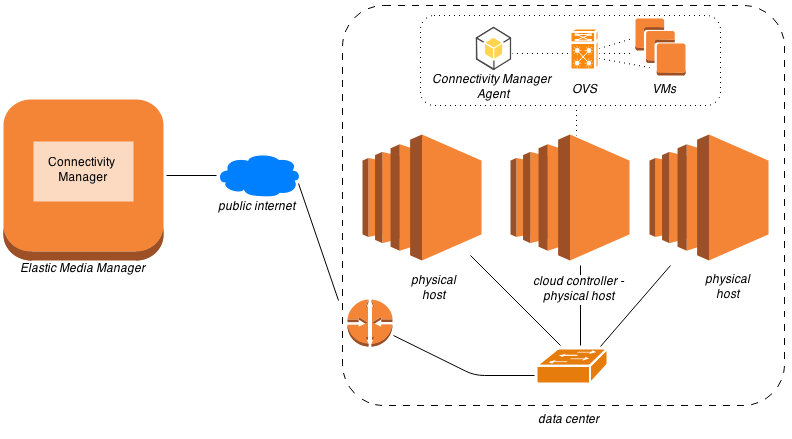
\includegraphics[width=0.8\textwidth]{images/design/scope_architecture.png}

\caption{Architectural overview}
\end{figure}

\newpage
In virtualized cloud infrastructure like OpenStack, the placement of Virtual Machines (VMs) on a particular compute node can be decided on by comparing different run-time parameters. The network connectivity between those VMs has to be prioritized and classified depending on the type of service that the server provides.

Currently there are a number of solutions for managing network connectivity between virtual servers that partially fit the requirements of this work. A comparison and their current limitations follows in the next section. The selected approach is the extension of existing network control and management services with Quality of Service (QoS) capabilities and the ability to choose a host for the deployment of the topology. In support of the thesis the Connectivity Manager will be implemented and the evaluation of the network performance will be performed on basis of the services of the NUBOMEDIA project.


\section{Overview}

\textbf{Chapter 1} begins with the motivation for this thesis and gives a brief introduction into the objectives and the scope.

\textbf{Chapter 2} gives an overview of traditional network concepts and a introduction to SDN and its components. Furthermore the different services that OpenStack consists of will be described.

\textbf{Chapter 3} conceptualizes the state-of-the-art solutions that are currently available and evaluates their implementation and limitations.

\textbf{Chapter 4} contains an analysis of requirements.

\textbf{Chapter 5} gives an architectural overview of the Connectivity Manager. Moreover design aspects are introduced and illustrated in relation to their requirements.

\textbf{Chapter 5} examines the implementation of the Connectivity Manager and Agent.

\textbf{Chapter 6} evaluates the network performance tests on the basis of one use-case.

\textbf{Chapter 7} summarizes the results of this work and gives an outlines possible future work.


